\documentclass{article}
\usepackage[utf8]{inputenc}

\title{Assignment 3: Minimax}
\author{Brian Jacobel}
\date{Artificial Intelligence, Fall 2013}

\usepackage{natbib}
\usepackage{graphicx}
\usepackage[margin=1in]{geometry}
\usepackage{setspace}
\usepackage{indentfirst}

\begin{document}

\maketitle

\begin{doublespace}

\section{Results}

\section{Discussion}

\subsection{Heuristics}

 
\subsection{Ordering}



\subsection{Columns}

\begin{figure}[ht!]
\centering
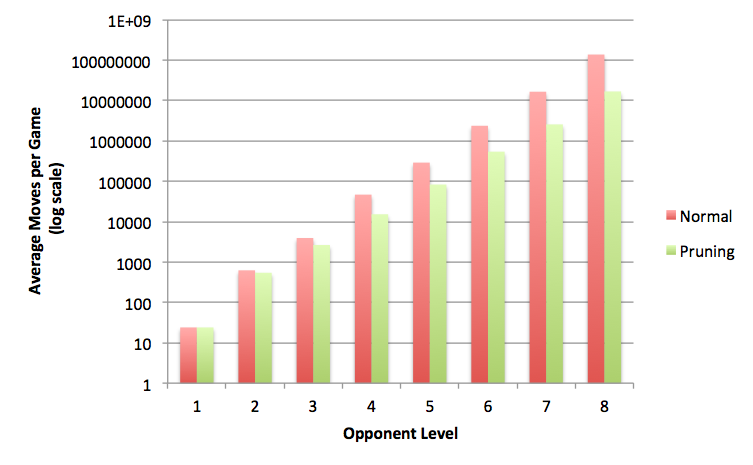
\includegraphics[width=6.5in]{../Data/Graphs/Graph2}
\caption{The average number of moves per game with pruning enabled and disabled at each of the eight opponent difficulty levels.}
\end{figure}

\begin{figure}[ht!]
\centering
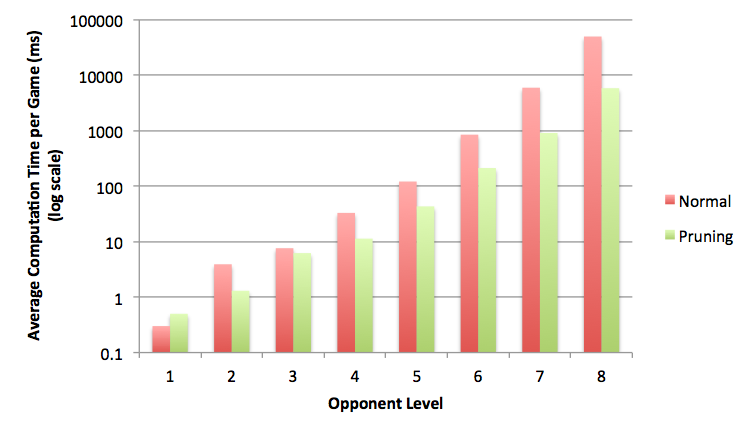
\includegraphics[width=6.5in]{../Data/Graphs/Graph3}
\caption{The average time spent exploring moves for the AI player per game with pruning enabled and disabled at each of the eight opponent difficulty levels.}
\end{figure}

\begin{figure}[ht!]
\centering
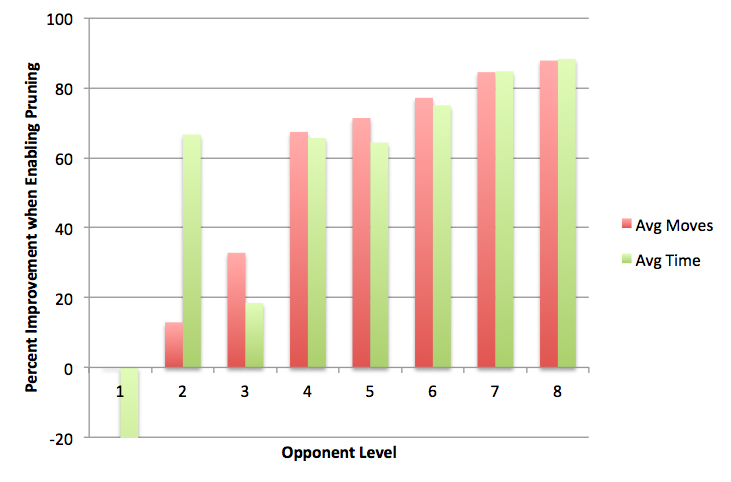
\includegraphics[width=6.5in]{../Data/Graphs/Graph1}
\caption{The effects on both the average number of moves and the average time when pruning is enabled, as compared to games at the same level with pruning disabled.}
\end{figure}


\end{doublespace}

\end{document}



